\section{Ficha de Avaliação de Software Educacional}

É consenso entre vários autores que a qualidade é uma meta no desenvolvimento de software a ser atingida. Uma das principais medidas é satisfazer
 as necessidades dos usuários além de atender determinadas propriedades e características da aplicação de acordo com seu contexto, ou seja,
 existem diferentes dimensões de qualidade e a importancia dos atributos ou características do software é variável segundo o domínio da aplicação \cite{rocha2008avaliaccao}.
 
A análise da qualidade de um software, além de abordar a base pedagógica, ou seja, a concepção teórica que descreve como o sujeito aprende, como ele se apropria e constrói seu
conhecimento deve levar em conta o ponto de vista técnico uma vez que estes aspectos orientam para uma adequada utilização. Nesse sentido fichas de avaliação de softwares
educacionais são propostas para auxiliarem no processo de avaliação do software \cite{vieira1999avaliaccao}. Dessa forma propomos a seguinte ficha para avaliação do eDesignPatterns:

\hspace*{-1.5in}
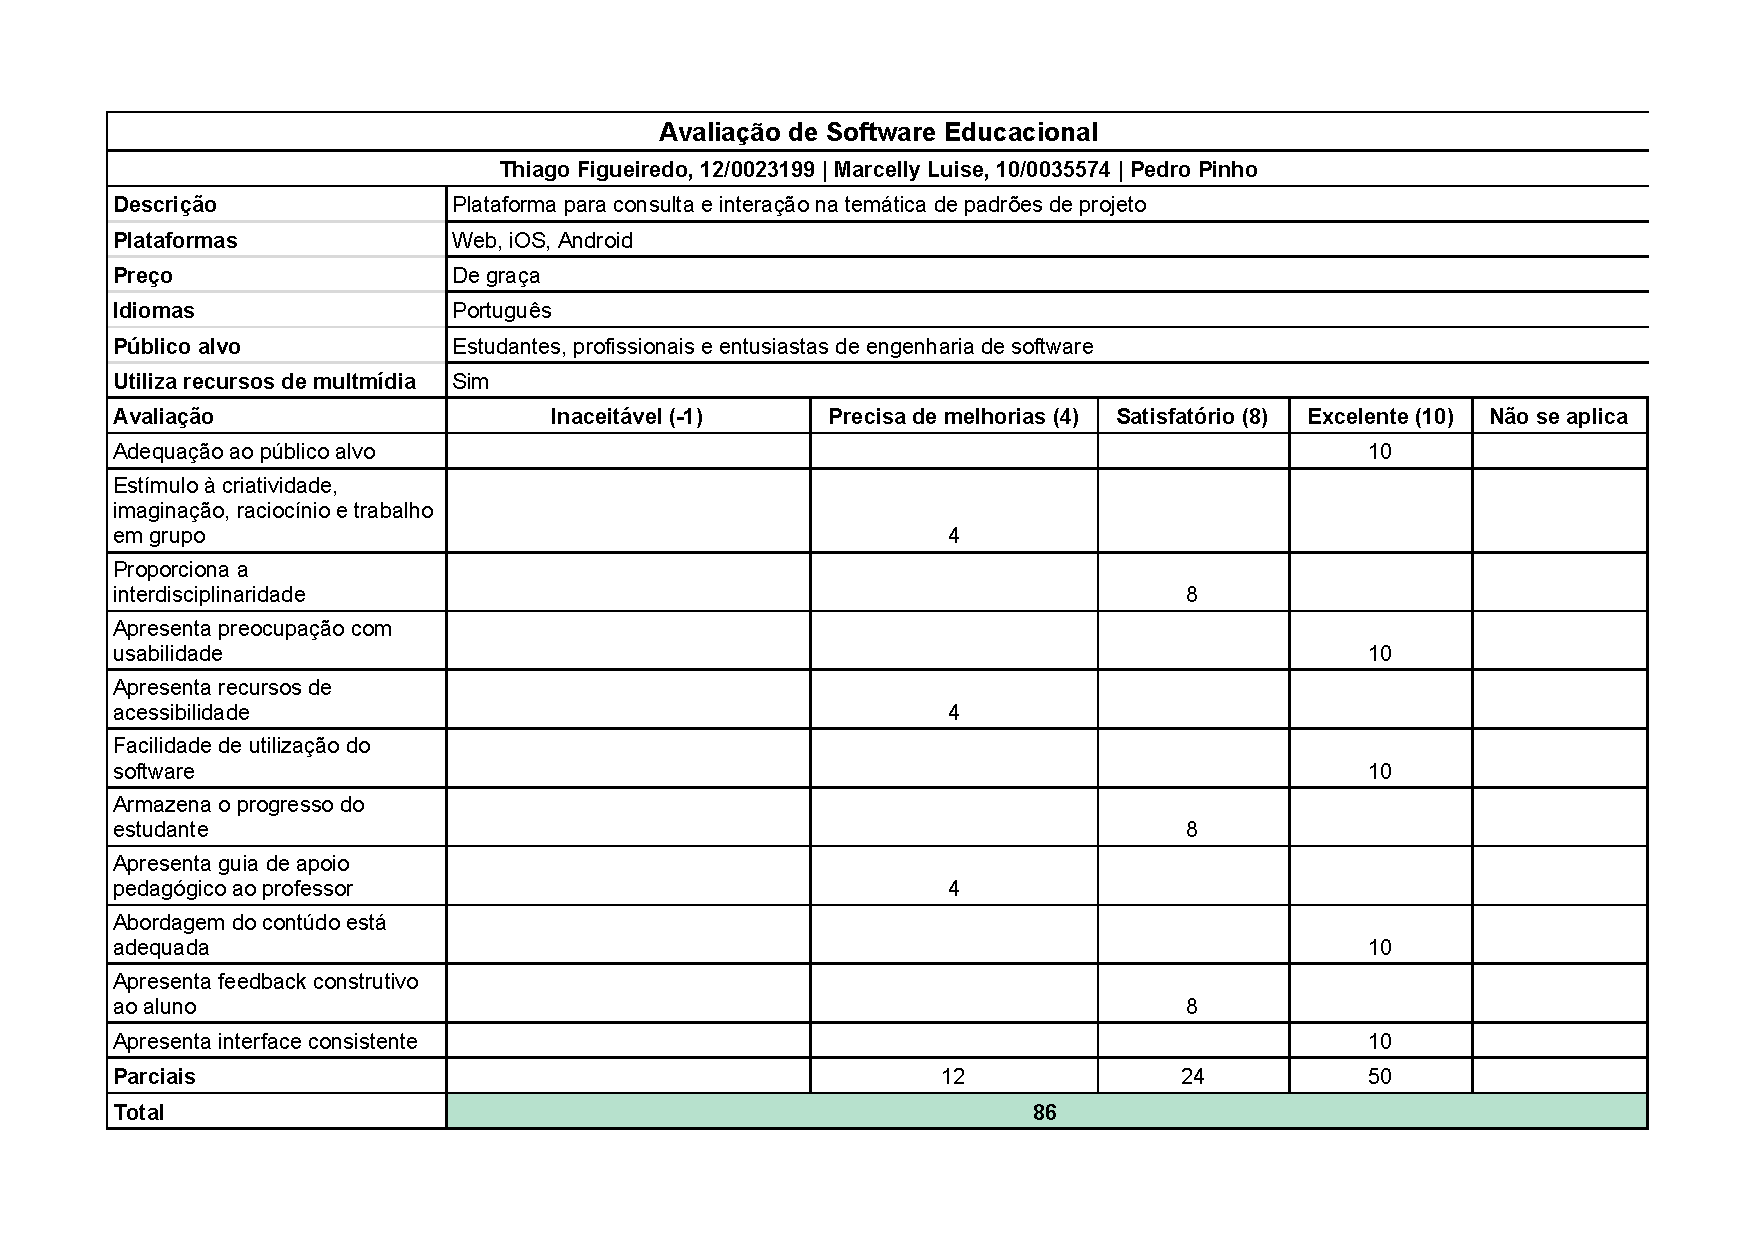
\includegraphics[width=630px]{fichaavaliacao.pdf}

